%!TEX root = ../report.tex
\section{Implementation}
The solution that has been proposed in the previous section is implemented using the C++ programming language in combination with the OpenGL API.
To program on the GPU, CG is used as shading language.

The actual SPH fluid simulation is given and can be seen in figure \ref{fig:sph}, by implementing the multiple passes described in the previous section, a nature like fluid is expected.
By creating Frame Buffer Objects (FBO), the results can be written to an off-screen rendering target.
This is useful since we are using multiple passes.
Also, multiple buffers can be attached to the FBO.

\subsection{Depth determination}
% TODO: Rephrase?
The depth at each pixel of each particle closest to the camera is determined using a combination of a vertex- and fragment shader.
Each particle has a position in world space that is passed to the vertex shader.
These particles are rendered as spheres to determine the correct depth values.

The vertex shader computes and passes the following properties of each particle to the fragment shader:
\begin{itemize}
 	\item Position of center in eye space.
 	\item Position of center in screen space.
 	\item Splat size.
 	\item Splat radius.
 \end{itemize} 

The fragment shader uses this input to determine the depth at every fragment.
To determine this depth, the splat is rendered as a sphere by discarding fragments that fall outside the sphere.
From this, the normal from the center of the sphere towards its surface is determined by taking the difference of the current fragment position and the current particle center.
Using this normal, the point is transformed to clip space, the $z$ value of this position is the depth value.
The depth values are then written to the depth buffer of the current FBO.

The depth component of each fragment can be visualized as grey value by setting the R, G and B components to the depth value.
The results of this visualization can be seen in figure \ref{fig:depth}.
It can be observed that the particles become darker when they appear  closer to the camera.

\begin{figure}[!th]
\hrule
\begin{center}
\vspace*{2ex}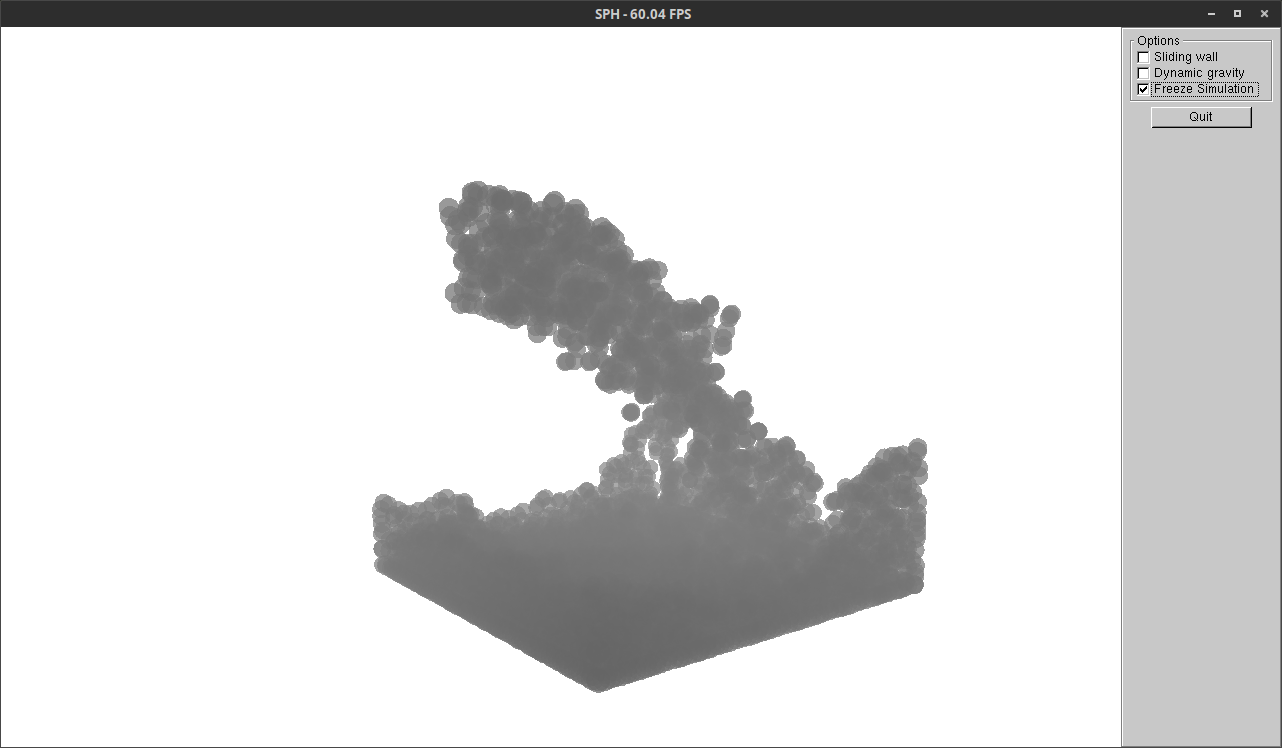
\includegraphics[width=0.48\textwidth]{pictures/depth.png}
\end{center}
\caption{Depth component visualization}
\label{fig:depth} 
\vspace*{2ex}
\hrule
\end{figure}

\subsection{Surface smoothing}
Two fragment shaders are used for surface smoothing.
The first fragment shader calculates the surface normals from the depth values and writes them in a texture.
The second fragment shader smooths the depth values using curvature flow, using the surface normals computed in the first shader.
These smoothed depth values are also written to a texture.

Since the smoothing happens in multiple steps, and textures can not be overwritten directly, multiple textures and FBOs are needed.
The depth texture has to be updated, so an extra temporary depth texture is needed, the same holds for the surface normal texture.
In each smooth step, one texture is used as input and the other is used as render target, the textures are switched after every step.
The surface normals change when the depth values are changed, so these also need to be recomputed every smooth step.
Listing \ref{program:smooth} shows this process in pseudocode.

\begin{algorithm}
	\begin{program}
	\caption
	|calculateNormals()|;
	\FOR i:=1 \TO |smoothSteps| \DO
		|smoothDepths()|;
		|calculateNormals()|;
		|flipTextures()|;
	\end{program}
	\label{program:smooth}
	\caption{Surface smoothing pseudocode}
\end{algorithm}

\subsubsection{Normal calculation}
The depth buffer is passed as input to the fragment shader, along with the uniform variables $C_x$ and $C_y$.
Since the depth buffer is in a texture, we can obtain the depth values of neighbours.
Using these neighbours, the finite differences between depth values can be calculated in the $x$ and $y$ direction.
Since we now have $C_x, C_y, \frac{\partial z}{\partial x}, \frac{\partial z}{\partial y}$ and $z$, we can calculate the normal according to equation \ref{eq:normals}.
These normals are written to the normals texture.

\subsubsection{Depth smoothing}
Since we now have all surface normals in a texture, finite differencing can be used again to calculate the derivatives of the surface normals.
The depth values are modified according to these derivatives and written to the depth texture.